%!TEX root = ../main.tex

\chapter{Related Works}
\label{chp:related}

Performing federated analytics tasks over genomics data requires a robust architecture composed by different layers: a federation layer that allows for multiple streaming connections with diverse and heterogeneous sources (relational, no-SQL and columnar \ac{DBMS}s); a virtualization layer that exposes "virtual" relational views of non-materialized data; an integration, ontology-based layer, so to add a semantic layer to the virtualized relational views, given the importance of exploring complex relationships among genomics data.

This approach has been formalized under the concept of \ac{OBDF} \cite{DBLP:conf/icde/GuCPLMX24}, and it is represented in Fig. \ref{fig:obdf}. As far as we know, no existing off-the-shelf system implementing this framework has ever been released: who intends to apply this architecture design have to manually install different components choosing among diverse competitors, and combining them together, dealing with possible underlying platform incompatibilities. Moreover, having no off-the-shelf solutions implies no solutions specifically tailored and optimized for dealing with genomics data.

\begin{figure}[ht]
    \centering
    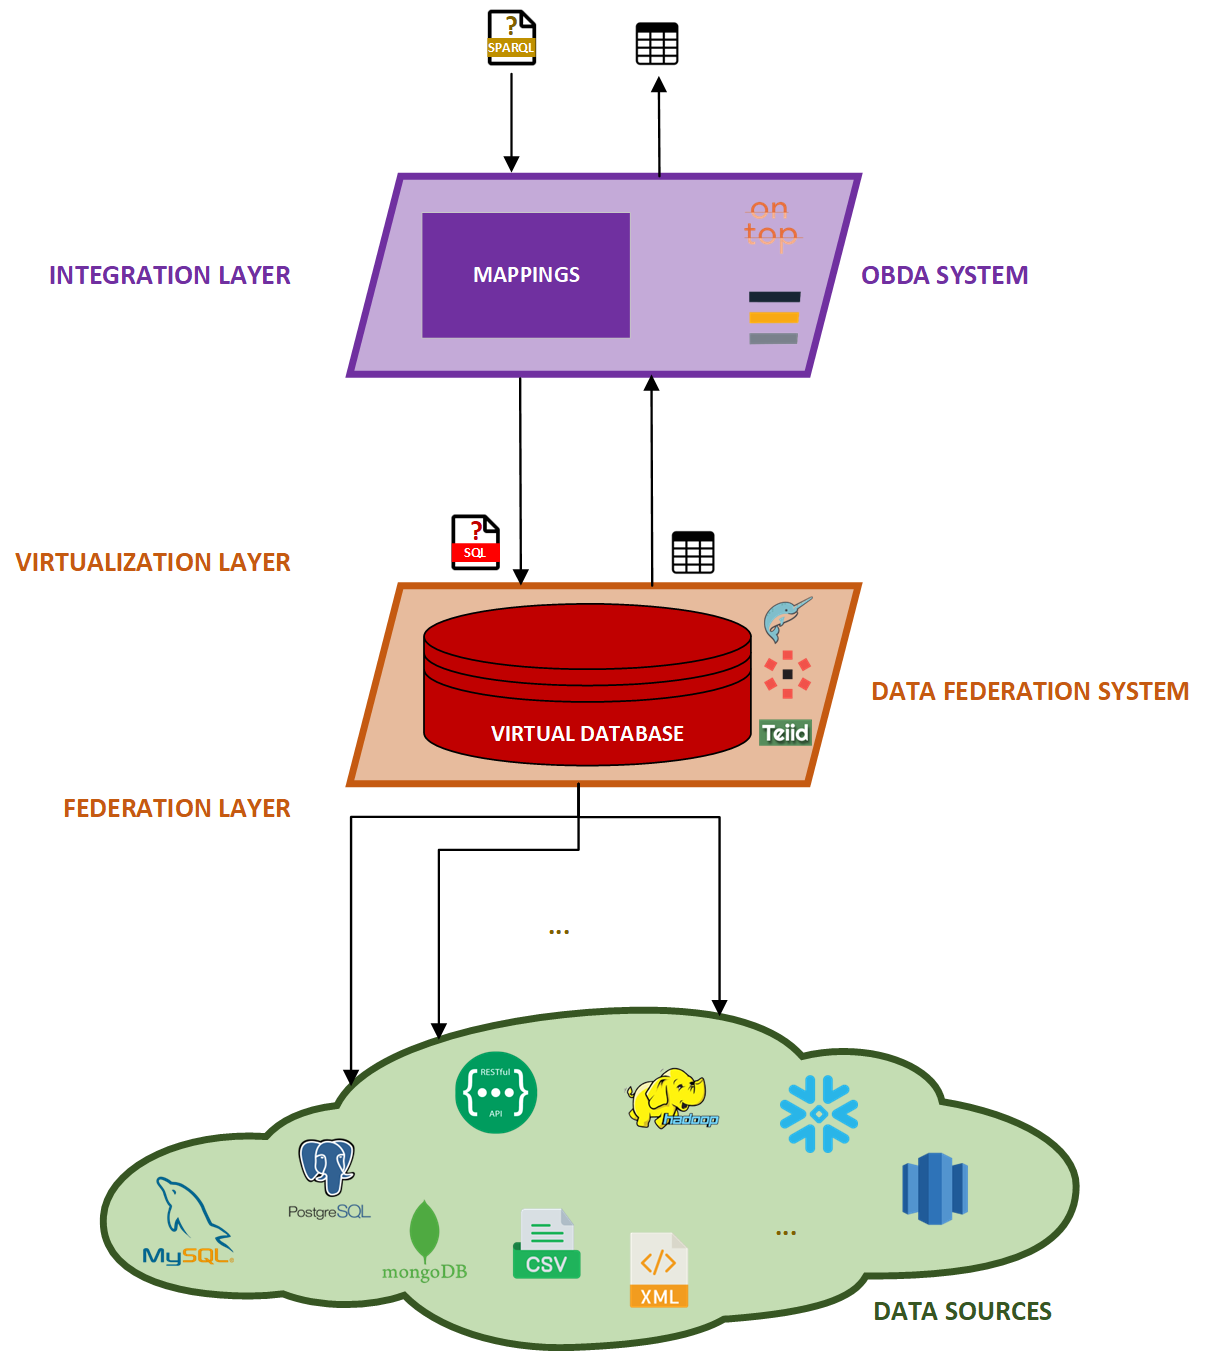
\includegraphics[width=11.5cm]{res/Drawing4.png}
    \caption{OBDF approach}
    \label{fig:obdf}
\end{figure}

Nonetheless, similar design proposal have been implemented in order to address both research questions as well as enterprise requirements. In this section, we will briefly discuss two solutions, one for each environment, analyzing them in details highlighting strengths and weaknesses.

\section{BigDAWG}
As an example addressing research questions about managing heterogeneous data we have BigDAWG \cite{DBLP:conf/hpec/GadepallyCDEHKM16}, developed under the Intel Science and Technology Center on Big Data. BigDAWG's architecture is composed of four layers: the base layer, the island layer, the main BigDAWG layer, and the application layer. Each layer serves a distinct purpose, from managing diverse physical data stores to facilitating user interaction through applications. This multi-layered approach allows BigDAWG to support various data models and query languages, thus offering a robust solution for cross-database queries and operations.
While traditional systems such as Garlic and IBM DB2 have demonstrated the capability to handle data across different storage systems using a unified interface, BigDAWG distinguishes itself by its comprehensive support for "islands" of different data models. This island approach not only supports operations across various data types but also enhances performance by optimizing queries based on the data model and the underlying database engine. This feature is critical in environments where performance and response times are crucial, such as in medical or real-time analytics applications.
Despite its advanced architecture and capabilities, BigDAWG is not without challenges. It is not available as an off-the-shelf solution; rather, it require certain levels of expertise if someone intends to install it or develop new islands modules. This means that significant effort would be required to adapt it to specific operational needs. Additionally, there is limited literature and empirical studies on its deployment in real-world scenarios, which poses doubts about considering its implementation.
In summary, while BigDAWG represents a significant advancement in the field of database management systems, its practical application is limited by the prototype nature of its current implementation and the lack of extensive real-world testing. Future research could focus on reducing the barrier to its adoption, refining its architecture based on operational feedback, and expanding its use cases across different scenarios to fully realize its potential.

\section{Optique}
Optique \cite{DBLP:journals/ws/KharlamovMSXKR19}, developed by Siemens, exemplifies an implementation of OBDA tailored to the industrial applications. Unlike conventional OBDA systems which typically focus on static data, Optique is designed specifically to handle both streaming and static data. This dual capability is crucial for environments like Siemens, where real-time data from sensors needs to be integrated with historical data for comprehensive analysis and monitoring.
Optique comprises many technologies: \ac{STARQL}, A language that supports complex queries over streaming and static data at the same time; ExaStream, A backend system optimized for low-latency queries on high-velocity streams; OptiqueVQS (Visual Query System), a component that improves usability by enabling users to formulate queries without prior knowledge of query languages.
Although it has advanced capabilities, Optique remains a proprietary system not available for public use, which limits its adoption outside Siemens. This exclusivity may impede broader validation and benchmarking against other OBDA systems in real-world settings.